%% Semplice beamer conforme al powerpoint ufficiale
%% dal sito di Ca' Foscari. Si basa sul tema "default"
%% mandate Modifiche e migliorie! Guido.Caldarelli@unive.it 
% Elenco Contributori 
% Guido Caldarelli, Matteo Brilli 

%\documentclass{beamer}
% decide below the aspect ratio between 16:9 and 4:3
%\documentclass[aspectratio=43]{beamer}
\documentclass[aspectratio=169, 11pt]{beamer}

\usepackage[utf8]{inputenc}
\usepackage{tikz}
\usepackage{multicol}
\usetikzlibrary{tikzmark, shapes}
\usepackage{bm}
\usepackage[dvipsnames]{xcolor}
\usepackage{graphicx}  % Required for \settowidth
\usepackage{appendixnumberbeamer}
% Questo tema commentato di sotto produce un beamer più tradizionale 
%\usetheme[secheader]{Boadilla}


%%%-----------------------------------------------------------%
%% Cambia colori da thema default
%% Questi sono i due colori ufficiali rosso e grigio
\definecolor {firebrick}{rgb}{0.709,0.196,0.329} 	%{ 181 ,50 ,84}
\definecolor {cfgrey}{rgb}{0.537,0.537,0.537} 	%{ 137,137,137}
\definecolor {cflink}{rgb}{0.615,0.615,0.607} 	%{157,157,155}
\definecolor {cfgreen}{rgb}{0.004, 0.196, 0.125} %{1, 50, 32}
\definecolor{firebrick}{HTML}{B22222} %firebrick 

\setbeamercolor{palette primary}{bg=firebrick,fg=white}
\setbeamercolor{palette secondary}{bg=firebrick,fg=white}
\setbeamercolor{palette tertiary}{bg=firebrick,fg=white}
\setbeamercolor{palette quaternary}{bg=firebrick,fg=white}
\setbeamercolor{palette five}{bg=cfgreen, fg=white}
\setbeamercolor{structure}{fg=firebrick}		 % itemize, enumerate, etc
\setbeamercolor{section in toc}{fg=firebrick} 		 % TOC sections
% Override palette coloring with secondary
\setbeamercolor{subsection in head/foot}{bg=cfgrey,fg=white}
%%%------------------------------------------------------------

%% Definisce il blocco con riquadro che non è presente nel tema default (commentare se si usano altri temi)
\setbeamercolor{uppercolor}{fg=white,bg=firebrick}%
\setbeamercolor{lowercolor}{fg=black,bg=white}%
\def \bblock{\begin{beamerboxesrounded}[upper=uppercolor,lower=lowercolor,shadow=true]}
\def \eblock{\end{beamerboxesrounded}}
%%-----------------------------------------------------------
%\setbeamertemplate{footline}[frame number]
% Customize the footline
\setbeamertemplate{footline}{%
  \leavevmode%
  \hbox to \paperwidth{%
    % First box (Email address) - Exactly 1/3 of paperwidth
    \begingroup
    \setlength{\fboxsep}{2pt}% Padding inside the box
    \colorbox{firebrick}{\makebox[\dimexpr0.333\paperwidth\relax][c]{\strut\textcolor{white}{\texttt{myp23@cam.ac.uk}}}}%
    \endgroup
    % Second box (Custom text) - Exactly 1/3 of paperwidth
    \begingroup
    \setlength{\fboxsep}{2pt}% Padding inside the box
    \colorbox{firebrick}{\makebox[\dimexpr0.333\paperwidth\relax][c]{\strut\textcolor{white}{K34}}}%
    \endgroup
    % Third box (Frame number) - Exactly 1/3 of paperwidth
    \begingroup
    \setlength{\fboxsep}{2pt}% Padding inside the box
    \colorbox{firebrick}{\makebox[\dimexpr0.334\paperwidth\relax][c]{\strut\textcolor{white}{\insertframenumber/\inserttotalframenumber}}}%
    \endgroup
  }%
  \vskip0pt%
}
\setbeamertemplate{caption}{\raggedright\insertcaption\par}
%% Intestazione ripetuta per ogni slide
\addtobeamertemplate{headline}{%
\vspace{0.25cm} \ \ 

\includegraphics[height=1.0cm]{Ca_Foscari Beamer/cambridge-cropped.pdf}

\includegraphics[height=1.0cm]{kicc.png} 	% sostituire con logobeamIT.png per italiano
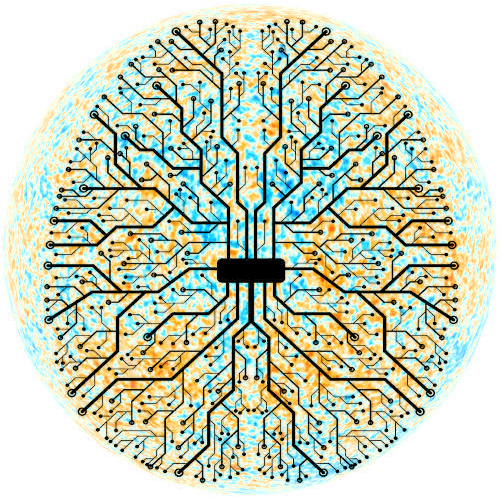
\includegraphics[height=1.0cm]{Ca_Foscari Beamer/handley-lab.png}
%\hspace{0.641\textwidth}{\color{cflink} {\small www.unive.it}} %per 16:9
%\hspace{0.551\textwidth}{\color{cflink} {\small www.unive.it}} %per 4::3
\vspace{0.25cm}
{\color{firebrick} \hrule \hrule  }
\textbf{}
}{}
%%-------------------------------------------------------------

%This block of code defines the information to appear in the Title page
%%%
\title[Inference techniques in gravitational-wave science ] %optional
{Inference techniques in gravitational-wave science \\ \vspace{0.5em}
\large Current and future prospects at Cambridge}
\author[Metha Prathaban] % (optional)
{Metha Prathaban} %\break %\vfill
\includegraphics[width=0.16\textwidth]{Ca_Foscari Beamer/qr-code.png}}
\date{}



\setbeamertemplate{frametitle}[default][right, rightskip=.5cm] {}
\addtobeamertemplate{frametitle}{\vspace*{-1.4cm}}{}
\setbeamertemplate{navigation symbols}{}
%End of title page configuration block
%------------------------------------------------------------


%------------------------------------------------------------
%The next block of commands puts the table of contents at the 
%beginning of each section and highlights the current section:

\AtBeginSection[]
{
  \begin{frame}
    \frametitle{Table of Contents}
    \tableofcontents[currentsection]
  \end{frame}
}
%------------------------------------------------------------

\begin{document}

%The next statement creates the title page.
\frame{\titlepage}
%---------------------------------------------------------
%This block of code is for the table of contents after
%the title page
% \begin{frame}
% \frametitle{About Me}
% \begin{itemize}
%     \item 3rd year PhD student
%     \item Work on Bayesian numerical method development in context of GWs
% \end{itemize}
% \vspace{2em}
% \bblock{\begin{center}
% Current work is in collaboration with Will Handley and Harry Bevins.
% \end{center}}
% \begin{center}
% 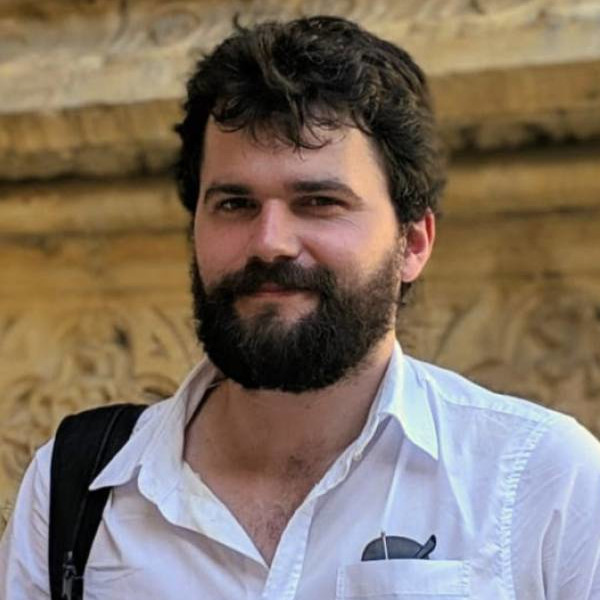
\includegraphics[height=2.0cm]{Ca_Foscari Beamer/will_handley.jpg}
% 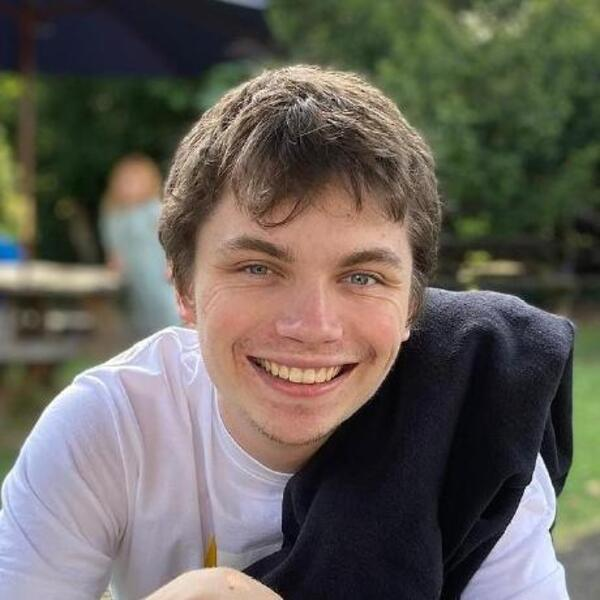
\includegraphics[height=2.0cm]{Ca_Foscari Beamer/harry_bevins.jpg}
% \end{center}
% \eblock
% \end{frame}
%This block of code is for the table of contents after
%the title page
\begin{frame}
\frametitle{Table of Contents}
\tableofcontents
\end{frame}
%---------------------------------------------------------


\section{Current landscape}


% \begin{frame}{Inverse problems}\vfill

%     \begin{tikzpicture}[node distance=5cm, auto]
%     % Nodes
%     \node (params) [draw, rectangle, rounded corners, minimum width=3cm, minimum height=1cm, align=center] {model parameters \\ $\boldsymbol{\theta}$};
    
%     \node (model) [draw, rectangle, minimum width=3cm, minimum height=2cm, align=center, right of=params] {quantitative model};
    
%     \node (data) [draw, rectangle, rounded corners, minimum width=3cm, minimum height=1cm, align=center, right of=model] {data (predicted) \\ \ $\mathbf{D}$};

%      % Straight arrow with customizable height and centered text
%     \draw[->, thick] 
%     ([yshift=0cm] params.east) -- ([yshift=0cm] model.west);
    
%     \draw[->, thick] 
%     ([yshift=0cm] model.east) -- ([yshift=0cm] data.west);

%       % Text above the second rectangle
%     \node at ([yshift=0.3cm] model.north) {\textbf{Forward problem}};
%     % \draw[->, thick] 
%     % ([yshift=-0.2cm] data.west) -- node[midway, below] {\textcolor{firebrick}{Inverse problem}} ([yshift=-0.2cm] model.east);

%     \node (params2) [draw, rectangle, rounded corners, minimum width=3cm, minimum height=1cm, align=center, below of=params, yshift=2cm] {model parameters, inferred \\ $\boldsymbol{\theta}_{\text{est}}$};
    
%     \node (model2) [draw, rectangle, minimum width=3cm, minimum height=2cm, align=center, below of=model, yshift=2cm] {quantitative model};

%     \node (data2) [draw, rectangle, rounded corners, minimum width=3cm, minimum height=1cm, align=center, below of=data, yshift=2cm] {data (observed) \\ \ $\mathbf{D}_\text{obs}$};

%       % Text above the second rectangle
%     \node at ([yshift=0.3cm] model2.north) {\textbf{Inverse problem}};

%      % Straight arrow with customizable height and centered text
%     \draw[->, thick, line width=1.0mm] 
%     ([yshift=0cm] params.east) -- ([yshift=0cm] model.west);
    
%     \draw[->, thick, line width=1.0mm] 
%     ([yshift=0cm] model.east) -- ([yshift=0cm] data.west);

%      % Straight arrow with customizable height and centered text
%     \draw[->, thick, line width=1.0mm] 
%     ([yshift=0cm] model2.west) -- ([yshift=0cm] params2.east);
    
%     \draw[->, thick, line width=1.0mm] 
%     ([yshift=0cm] data2.west) -- ([yshift=0cm] model2.east);


%     % % Not equal signs (≠) between vertical pairs of rectangles (ensure correct syntax for \visible)
%     \visible<2>{\node at (data -| data2) [yshift=-1.4cm] {\textcolor{red}{$\boldsymbol{\neq}$ (observational error)}};}
%     \visible<2>{\node at (params -| params2) [yshift=-1.4cm] {\textcolor{red}{$\boldsymbol{\neq}$ (error propagation)}};}
    
% \end{tikzpicture}

% \end{frame}

\begin{frame}{The data}
 \begin{minipage}{0.55\textwidth} \vspace{0.5cm}
 \bblock{\centering LVK data so far}
\begin{itemize} 
\item \textbf{Short-duration signals from compact binary coalescences (CBCs)}
\item End of O3: $\approx 90$ confident detections  
\item End of O4a: $\approx 200$ confident detections 
\item Detection rate: $\approx 1$ every few days 
    \begin{itemize}
        \item Signals not overlapping
    \end{itemize}
\item BBH mergers last seconds, BNS mergers last minutes
    \begin{itemize}
        \item Short chunks of time to do PE on
    \end{itemize}
\item Computationally intensive to analyse, but doable with current pipelines.
\end{itemize} 
\eblock
\end{minipage}\hfill                                               \begin{minipage}{0.4\textwidth}\vspace{0.8cm}                          \centering                                          
    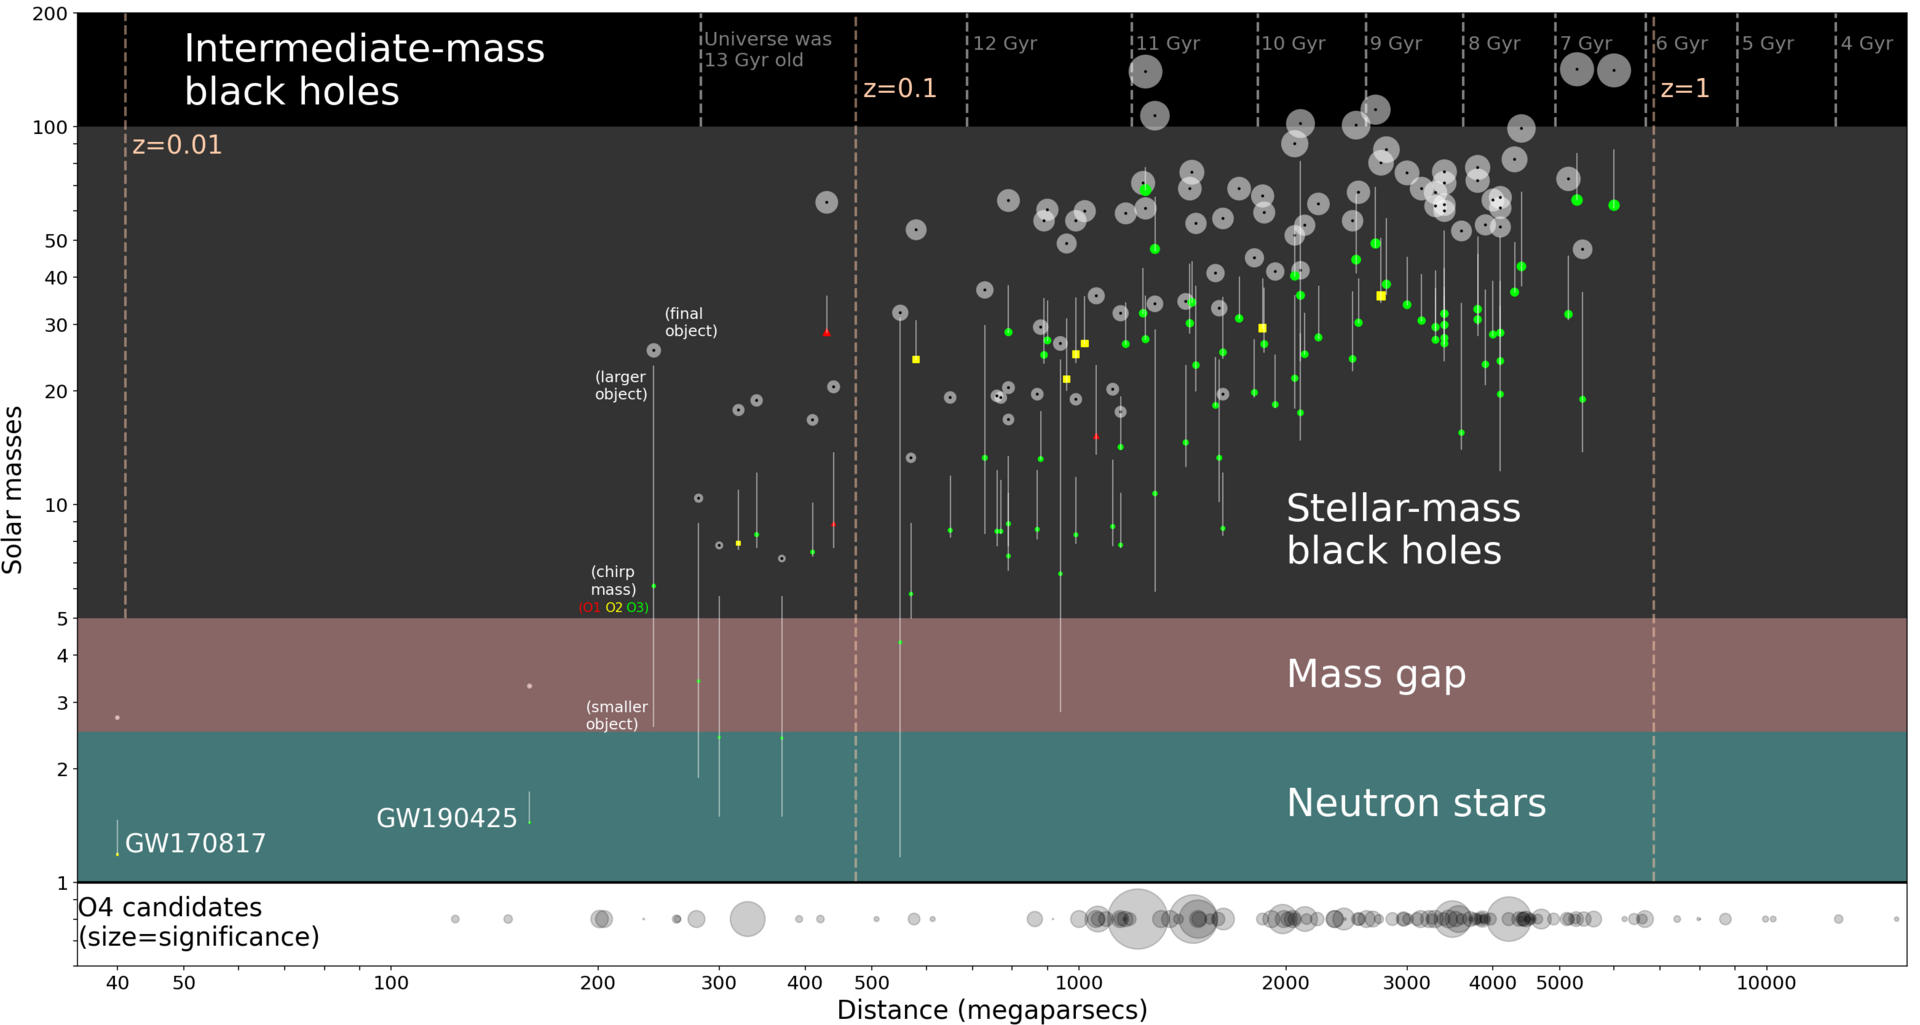
\includegraphics[width=\textwidth]{Ca_Foscari Beamer/GW_events_O3.png} \vfill
    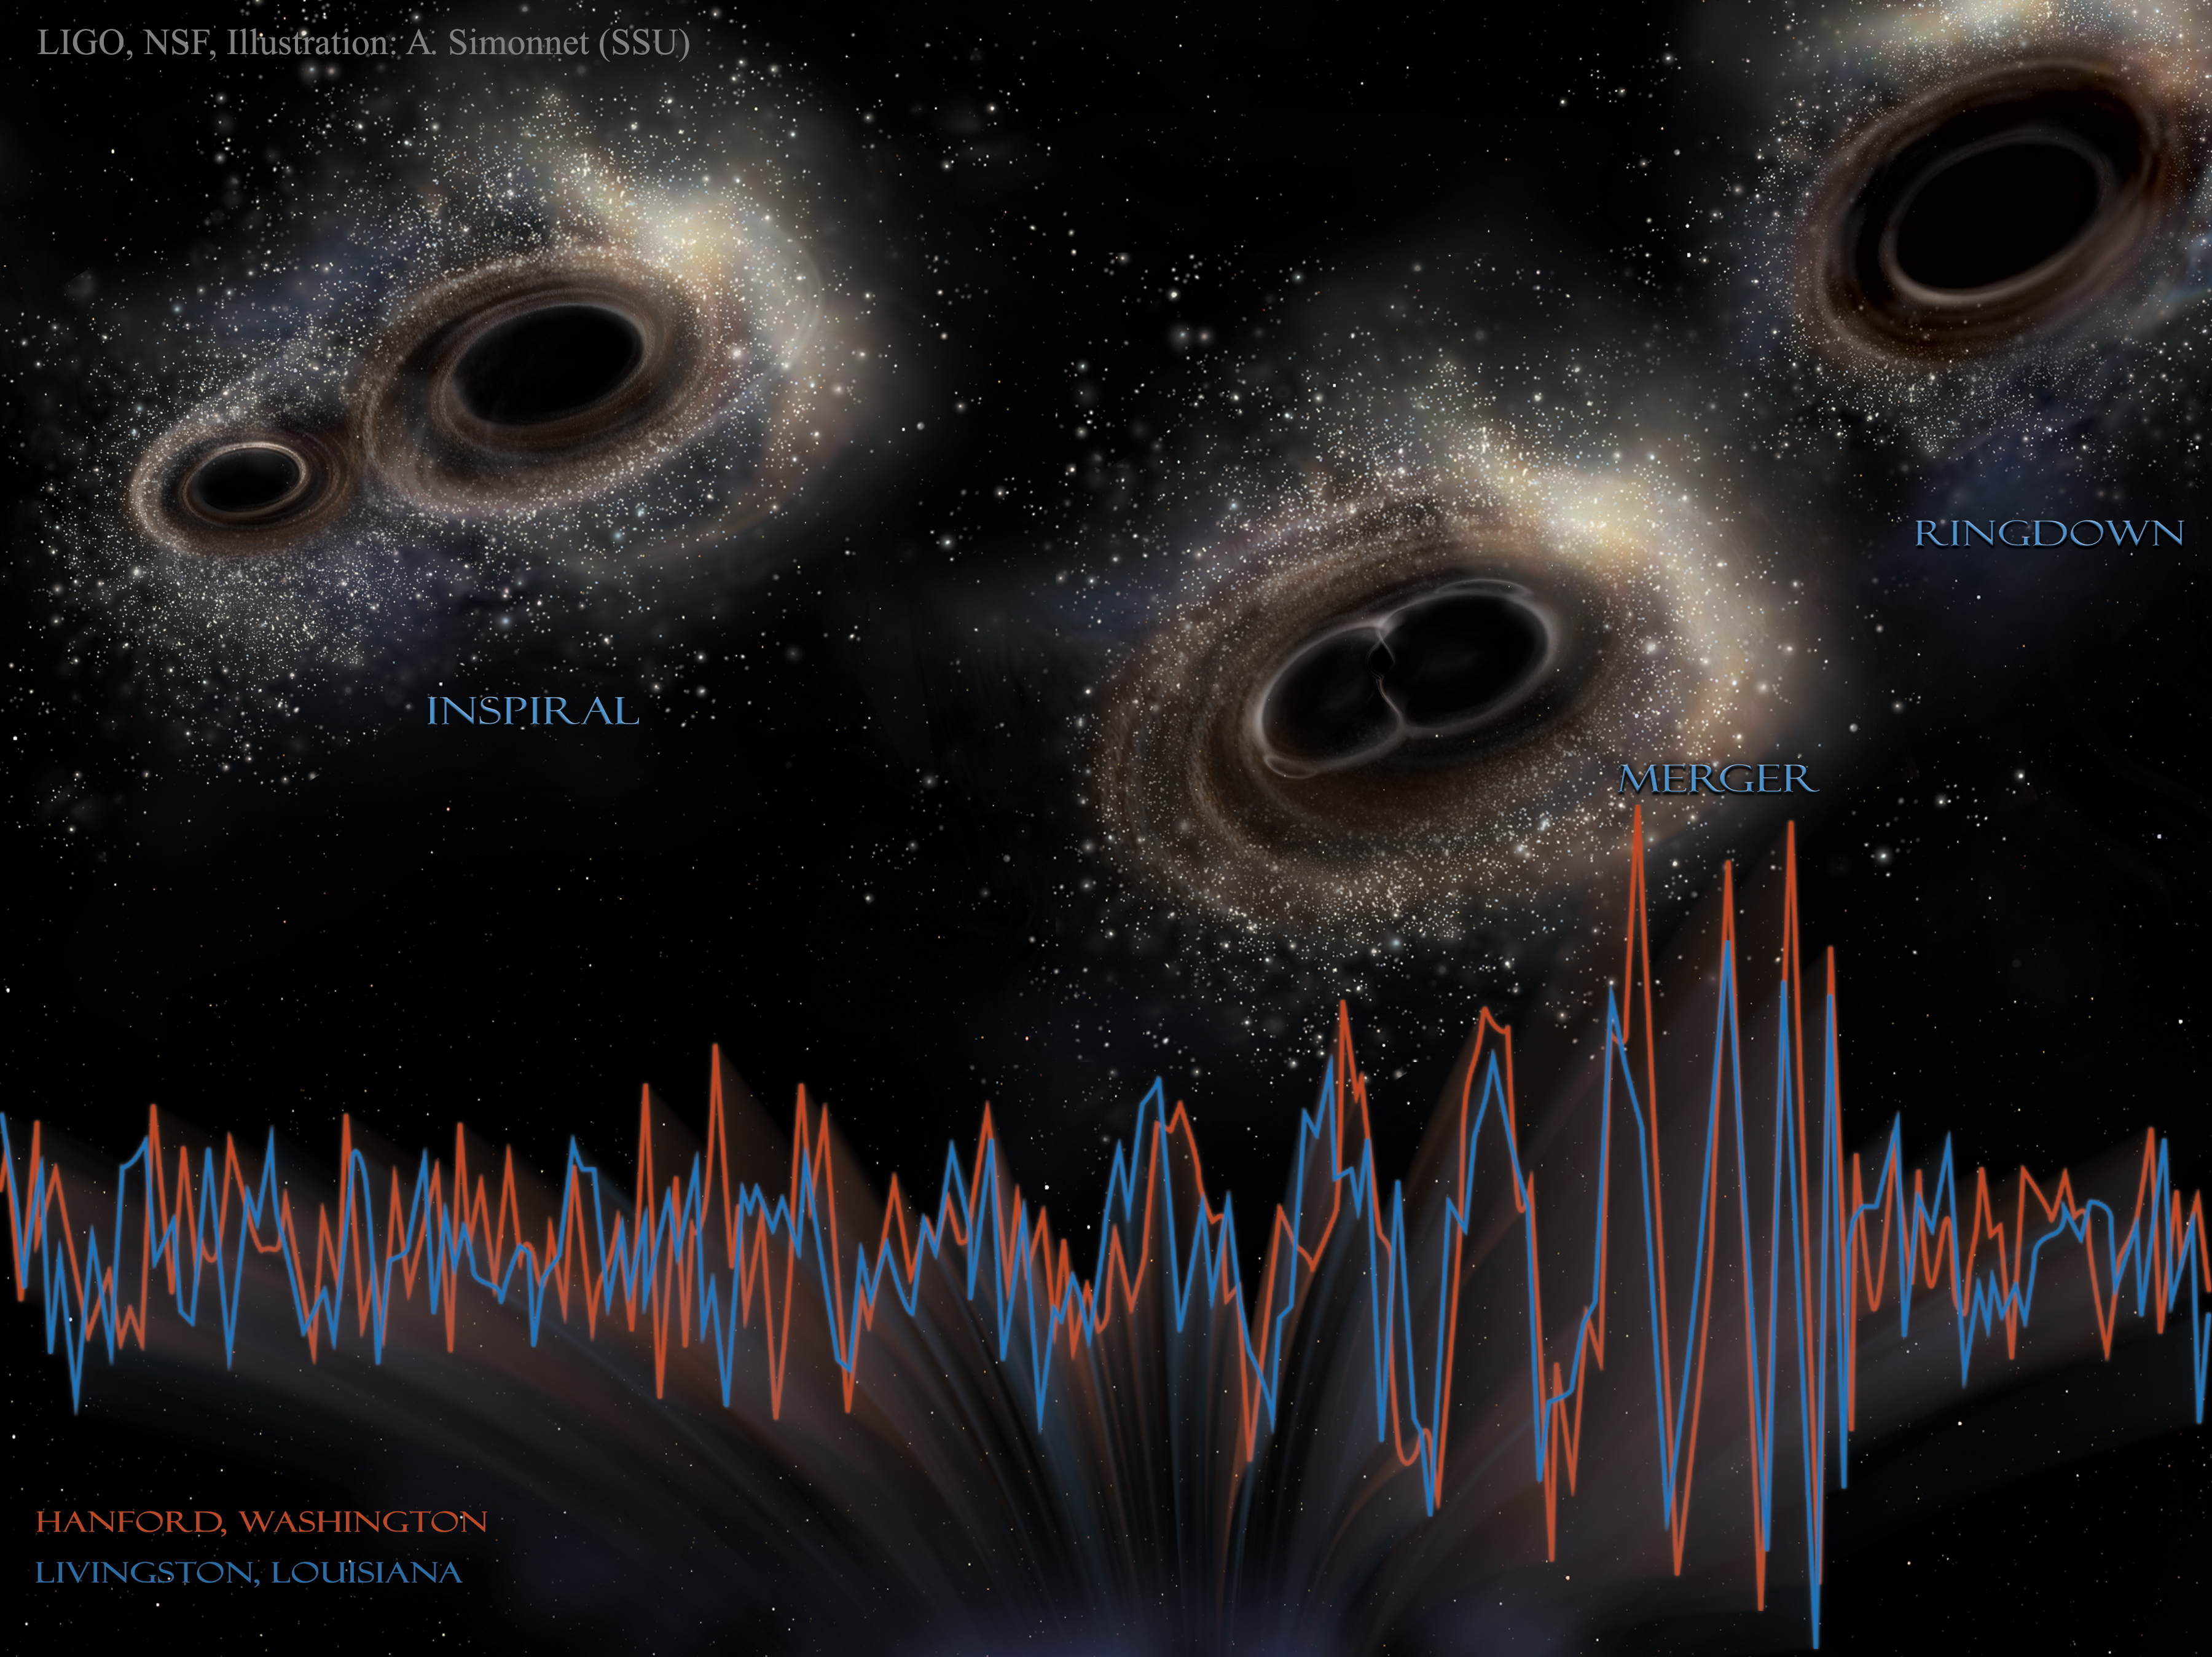
\includegraphics[width=0.7\textwidth]{Ca_Foscari Beamer/BH_merger.jpg}
\end{minipage}                                                    
\end{frame}

\begin{frame}{The analysis}
\begin{minipage}{0.6\textwidth}
\vspace{1cm}
    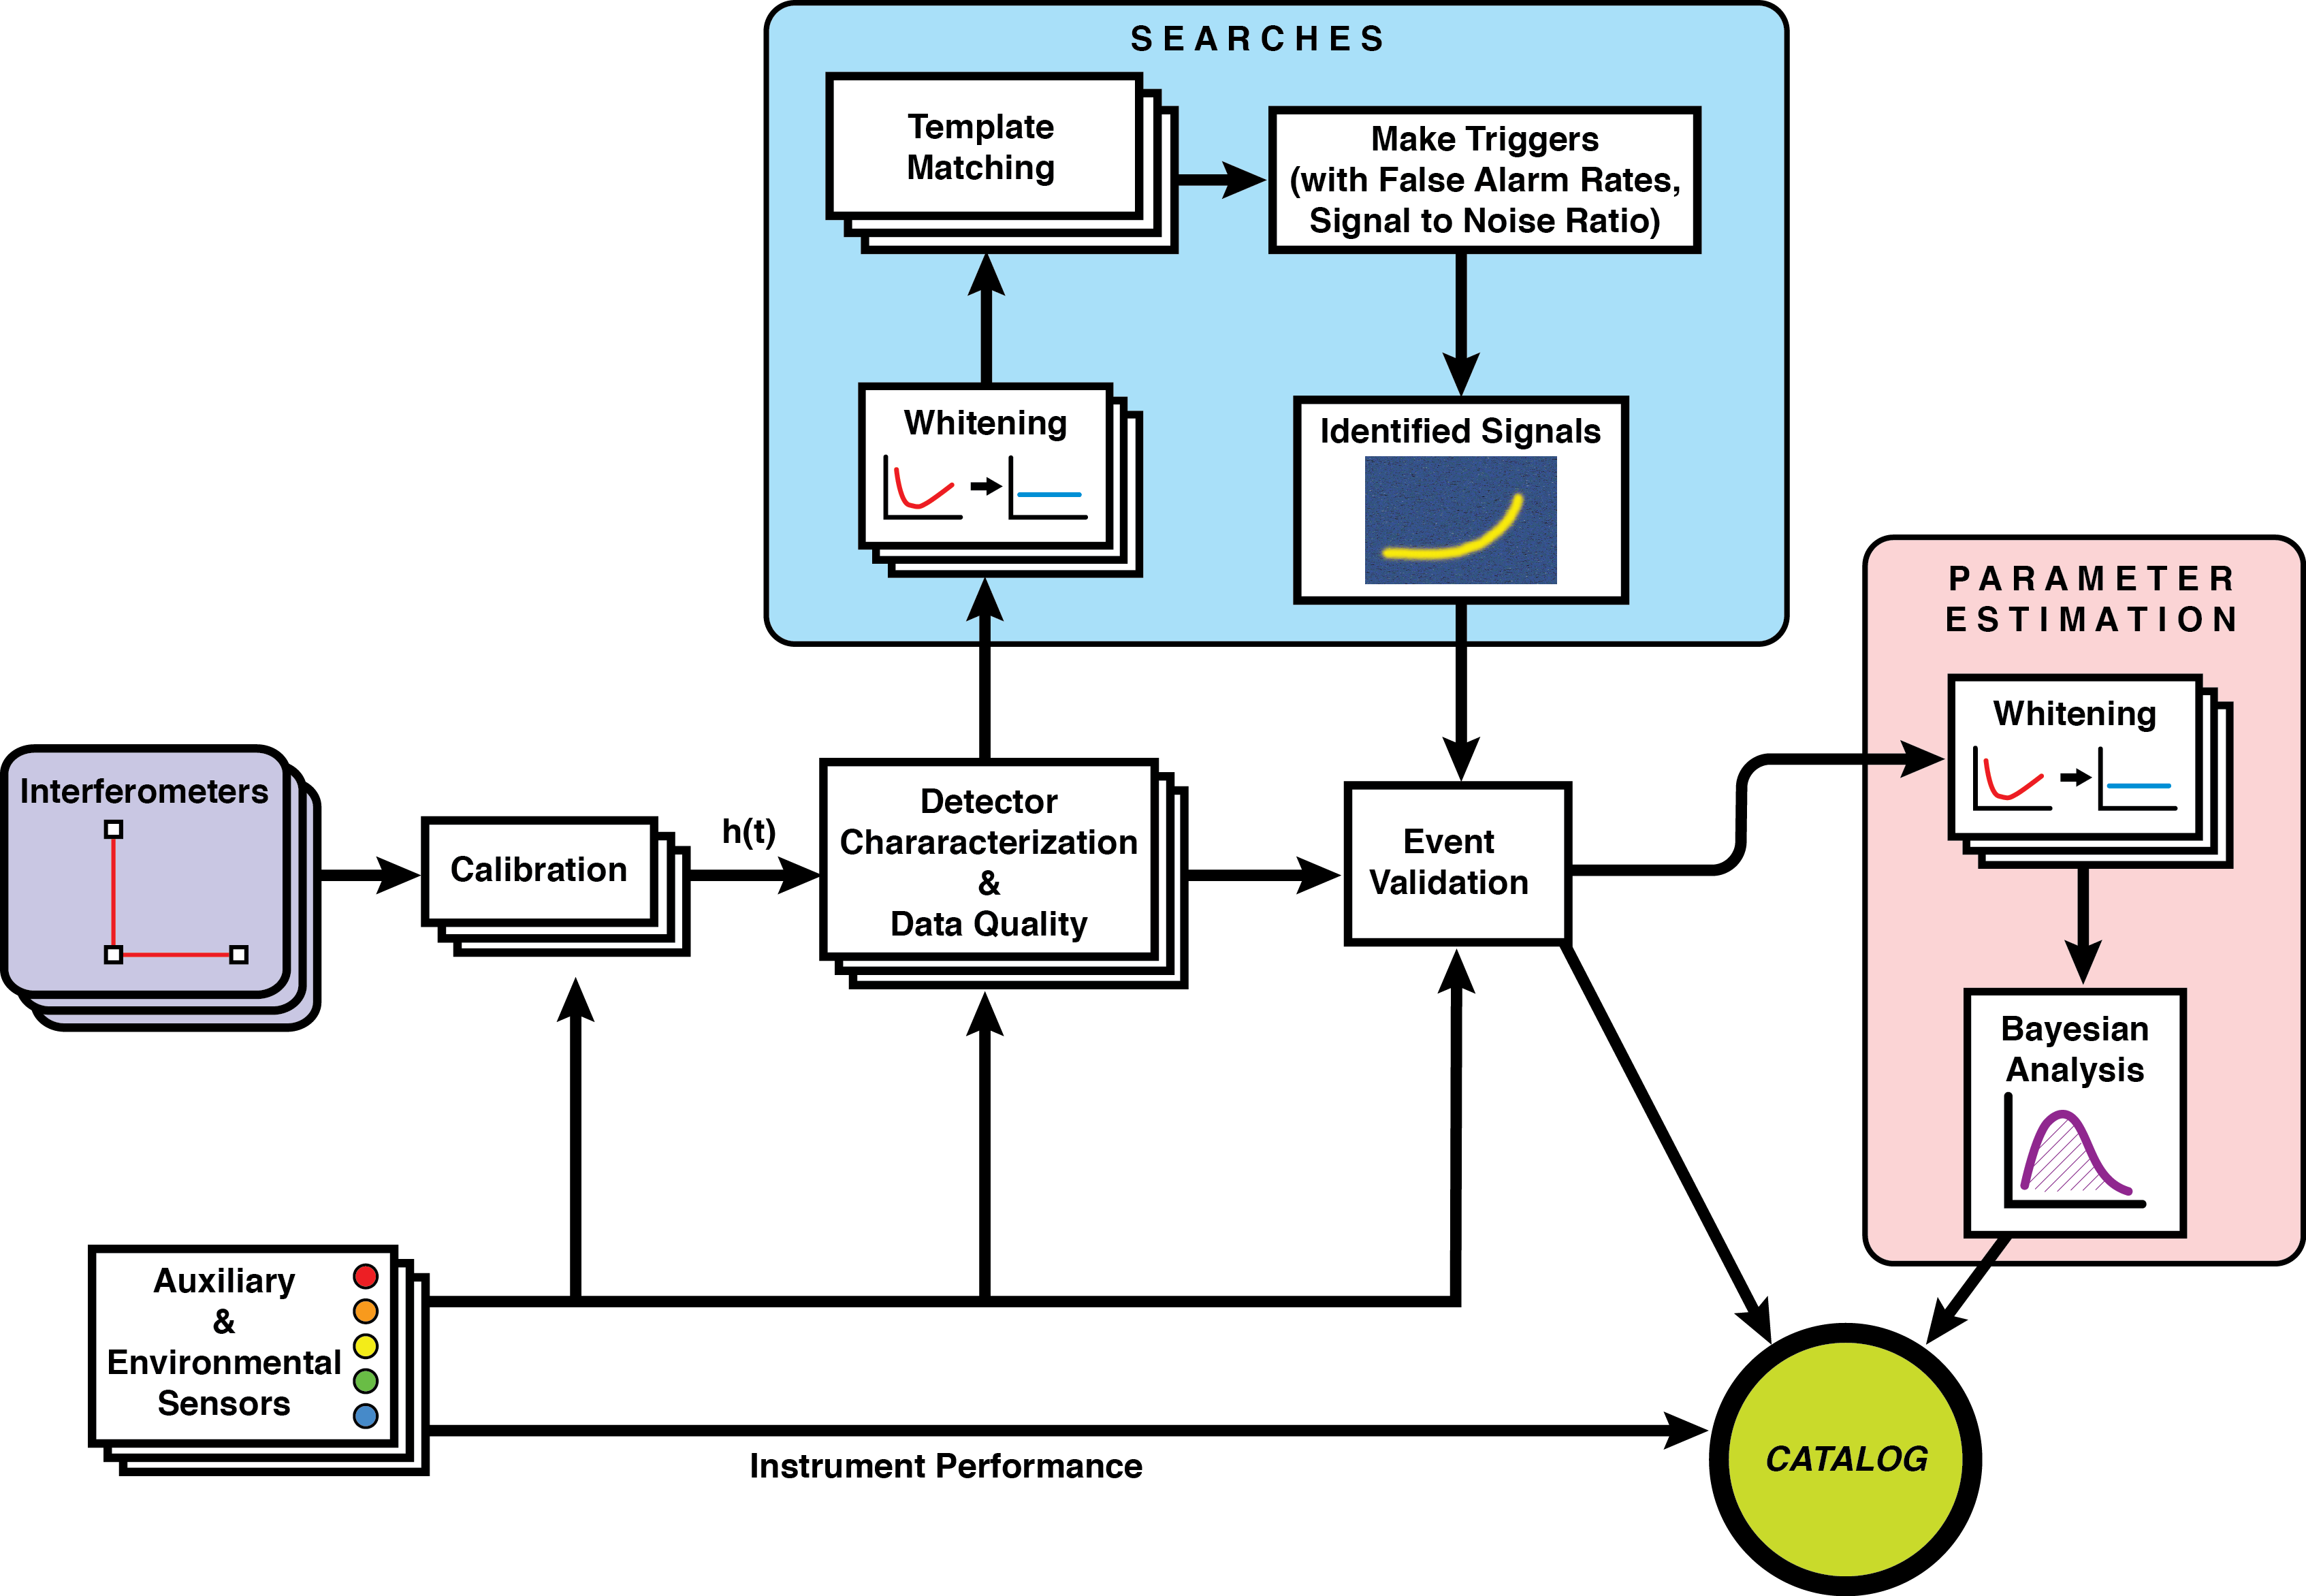
\includegraphics[width=\textwidth]{Ca_Foscari Beamer/lvk_analysis_pipeline.png}
    \tiny 1908.11170
\end{minipage}\hfill
\begin{minipage}{0.3\textwidth}\vspace{0.5cm}
    \begin{itemize}
        \item Pre-processing
            \begin{itemize}
                \item Calibration
                \item Noise characterisation
                \item Data quality checks
            \end{itemize}
        \item Detection
            \begin{itemize}
                \item Search pipelines: matched filter, un-modelled and stochastic.
            \end{itemize}
        \item Parameter estimation
        \item Model comparison
    \end{itemize}
\end{minipage}
\end{frame}

\begin{frame}{Matched Filtering}
\begin{minipage}{0.55\textwidth}\vspace{1em}
\bblock{Model comparison}
$\mathcal{H}_0$: Data contains noise \textbf{n} alone. \\
$\mathcal{H}_1$: Data contains noise \textbf{n} + signal \textbf{h}. \\

By Bayes' theorem: {\tiny 1908.11170} \\ 
     \begin{align}
         p(\mathcal{H}_1 | \textbf{d}) &= \frac{p(\mathcal{H}_1) p(\textbf{d} | \mathcal{H}_1)}{p(\mathcal{H}_0) p(\textbf{d} | \mathcal{H}_0) + p(\mathcal{H}_1) p(\textbf{d} |\mathcal{H}_1)} \\
&= \frac{p(\textbf{d} | \mathcal{H}_1)}{p(\textbf{d} | \mathcal{H}_0)} \biggl[ \frac{p(\textbf{d} | \mathcal{H}_1)}{p(\textbf{d} | \mathcal{H}_0)} +
\frac{p(\mathcal{H}_0)}{p(\mathcal{H}_1)} \biggr]^{-1}
\end{align}
\eblock
\end{minipage}
\hspace{1em}
\begin{minipage}{0.4\textwidth} \vspace{0.2cm}
\begin{block}{}
\begin{itemize}
    \item Monotonic in likelihood ratio $\Lambda(\textbf{d}|\boldsymbol{\theta}) = p(\textbf{d} | \mathcal{H}_1) / p(\textbf{d} | \mathcal{H}_0)$.
    \item  For Gaussian noise, $\log\Lambda(\textbf{d}|\boldsymbol{\theta}) \propto (\textbf{d} | \textbf{h}(\boldsymbol{\theta}))$ (the \textbf{matched filter}
\end{itemize}
\end{block}
\begin{block}{Template Banks}
    \begin{itemize}
        \item Construct bank of templates \textbf{h} with different source parameters $\boldsymbol{\theta}$.
        \item Compute maximum SNR across template bank and compare to threshold.
    \end{itemize}
\end{block}
\end{minipage}
\end{frame}



\begin{frame}{Parameter estimation}
     \begin{block}{Bayes' theorem for PE}
    \begin{equation}
       \mathcal{P}(\theta | \textbf{d}, \mathcal{M}) = \frac{P(\textbf{d} | \theta, \mathcal{M}) P(\theta | \mathcal{M})}{P(\textbf{d} | \mathcal{M})} = \frac{\mathcal{L}(\textbf{d} | \theta) \pi(\theta)}{\mathcal{Z}}
    \end{equation}
    \end{block}

    \begin{block}{Likelihood}
    Detector data modeled as sum of CBC signal, $\textbf{h}$, and noise, $\textbf{n}$. {\tiny 1809.02293}

    For stationary, Gaussian noise, with zero mean and a known covariance, $\Sigma_n$ : \\
    \begin{equation}
        \mathcal{L}(\textbf{d} | \theta) = \frac{1}{\sqrt{|2\pi\Sigma_n|}} \textrm{exp}\left(-\frac{1}{2} |\textbf{d} - \textbf{h}(\theta)|^T \Sigma_n^{-1} |\textbf{d} - \textbf{h}(\theta)| \right).
    \end{equation}
    \end{block}
\end{frame}

% \begin{frame}{Likelihood}
%     \begin{block}{}
%         Likelihood evaluation typically carried out in frequency domain. \vfill
%          % reference eric thrane Bayesian analysis intro paper
%         \begin{itemize}
%             \item Fourier transform the strain time series, $d(t)$.
%             \item In each frequency bin $j$, noise is characterized by one-sided noise power spectral density $P(f)$:
%             \begin{equation}
%                 \mathcal{L}(d_j | \theta) = \frac{1}{2\pi P_j} \textrm{exp}\left(-2 \Delta f \frac{|d_j - h_j(\theta)|^2}{P_j} \right ).
%             \end{equation}
%             \item Noise in each bin assumed to be independent so combined likelihood is product of likelihoods for each bin.
%             \item Combining data from different detectors is like combining data from different frequency bins.
%         \end{itemize}
%     \end{block}
% \end{frame}

\begin{frame}{Generating \textbf{h}}
    \begin{block}{Waveform Model}
        \begin{itemize}
            \item Numerical relativity is expensive!
            \item Models used in data analysis based on perturbative solutions, effective-one-body (EOB) waveforms, or phenomenological approaches. 
            \item 15 physical parameters for quasi-circular + generic spin vectors (11 for aligned spin) + extra for tidal effects for NS mergers.
        \end{itemize}
    \end{block}
    \begin{block}{Calibration Uncertainties}
    \begin{itemize}
        \item Uncertainties in amplitude and phase response of detectors are modeled and sampled over.
    \end{itemize} 
\end{block}
\end{frame}

\begin{frame}{Bayesian inference}
\begin{columns}
    
\column{0.5\textwidth}
\begin{itemize}
    \item Define \textcolor{BurntOrange}{prior}, \textbf{sample} (unnormalized) \textcolor{RoyalBlue}{posterior} ($\mathcal{L}(\textbf{d} | \theta) \times \pi(\theta)$).
    % \item Cannot plot full posterior distribution but can plot 1D and 2D \textbf{marginal} distributions (e.g. $\mathcal{P}(\mathcal{M}, q, \chi_\text{eff} | D)$) by integrating over all other parameters.
\end{itemize}
\vspace{2em}
\raggedright
Challenges:\vfill
    \begin{itemize}
        \item High-dimensional parameter spaces $\Rightarrow$ \textcolor{RoyalBlue}{posterior} occupies vanishingly small region of \textcolor{BurntOrange}{prior}.
        \item Complex waveform models with high costs
    \end{itemize}
    \vfill 

\column{0.5\textwidth}\
\vspace{-2em}
\centering
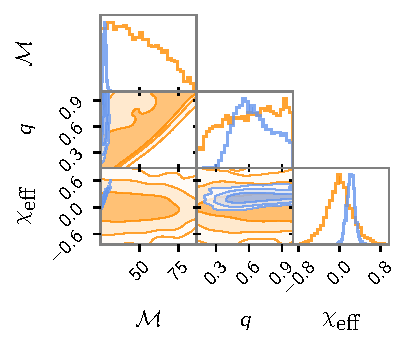
\includegraphics[]{Ca_Foscari Beamer/presentation_triangleplot.pdf}
\end{columns}
\end{frame}

% reference Will for this slide
\begin{frame}{Sampling}
    \begin{columns}
        \column{0.48\textwidth}
        \begin{block}{\textbf{MCMC}}
            % \only<16>{
            %     \begin{itemize}
            %         \item Single ``walker'', exploring posterior
            %         \item Fast, if proposal matrix is tuned
            %         \item Parameter estimation
            %     \end{itemize}
            % }
        \end{block}
            \includegraphics<1>[width=0.8\textwidth,page=16]{Ca_Foscari Beamer/himmelblau.pdf}%
            \includegraphics<2>[width=0.8\textwidth,page=17]{Ca_Foscari Beamer/himmelblau.pdf}%
            \includegraphics<3>[width=0.8\textwidth,page=18]{Ca_Foscari Beamer/himmelblau.pdf}%
            \includegraphics<4>[width=0.8\textwidth,page=19]{Ca_Foscari Beamer/himmelblau.pdf}%
            \includegraphics<5>[width=0.8\textwidth,page=20]{Ca_Foscari Beamer/himmelblau.pdf}%
            \includegraphics<6-15>[width=0.8\textwidth,page=21]{Ca_Foscari Beamer/himmelblau.pdf}%
        \centerline{\includegraphics<16>[width=0.5\textwidth,page=19]{Ca_Foscari Beamer/himmelblau.pdf}}
        \column{0.48\textwidth}
        \begin{block}<7->{\textbf{Nested sampling}}
            % \only<16>{
            %     \begin{itemize}
            %         \item Ensemble of ``live points''
            %         \item Slower than  MCMC methods
            %         \item Parameter estimation + model comparison
            %     \end{itemize}
            % }
        \end{block}
            \includegraphics<7|handout:0>[width=0.8\textwidth,page=1]{Ca_Foscari Beamer/himmelblau.pdf}%
            \includegraphics<8|handout:0>[width=0.8\textwidth,page=2]{Ca_Foscari Beamer/himmelblau.pdf}%
            \includegraphics<9|handout:0>[width=0.8\textwidth,page=3]{Ca_Foscari Beamer/himmelblau.pdf}%
            \includegraphics<10          >[width=0.8\textwidth,page=4]{Ca_Foscari Beamer/himmelblau.pdf}%
            \includegraphics<11|handout:0>[width=0.8\textwidth,page=5]{Ca_Foscari Beamer/himmelblau.pdf}%
            \includegraphics<12|handout:0>[width=0.8\textwidth,page=6]{Ca_Foscari Beamer/himmelblau.pdf}%
            \includegraphics<13|handout:0>[width=0.8\textwidth,page=7]{Ca_Foscari Beamer/himmelblau.pdf}%
            \includegraphics<14|handout:0>[width=0.8\textwidth,page=8]{Ca_Foscari Beamer/himmelblau.pdf}%
            \includegraphics<15|handout:0>[width=0.8\textwidth,page=15]{Ca_Foscari Beamer/himmelblau.pdf}%
        \centerline{\includegraphics<16>[width=0.5\textwidth,page=4]{Ca_Foscari Beamer/himmelblau.pdf}} 
    \end{columns}
\end{frame}

\section{Future landscape}

\begin{frame}{The data (ground-based)}
\begin{columns}
    \column{0.7\textwidth} \vspace{1cm}
    \bblock{\centering ET + CE}
    \begin{itemize}
        \item Ten-fold improvement in sensitivity compared to 2G detectors
        \item Detection rate: $\approx 10^5-10^6$ BBH and $\approx 7 \times 10^4$ BNS mergers per year
        \item Wider frequency band $\Rightarrow$ more intermediate mass BHs
        \item Improved localization
        \item Significantly higher SNR
        \item Longer signal durations %talk about noise
        \begin{itemize}
            \item Overlapping signals expected
        \end{itemize}
        \item New GW sources
    \end{itemize}
    \eblock

    \vspace{1cm}
    \column{0.3\textwidth}
    \centering
    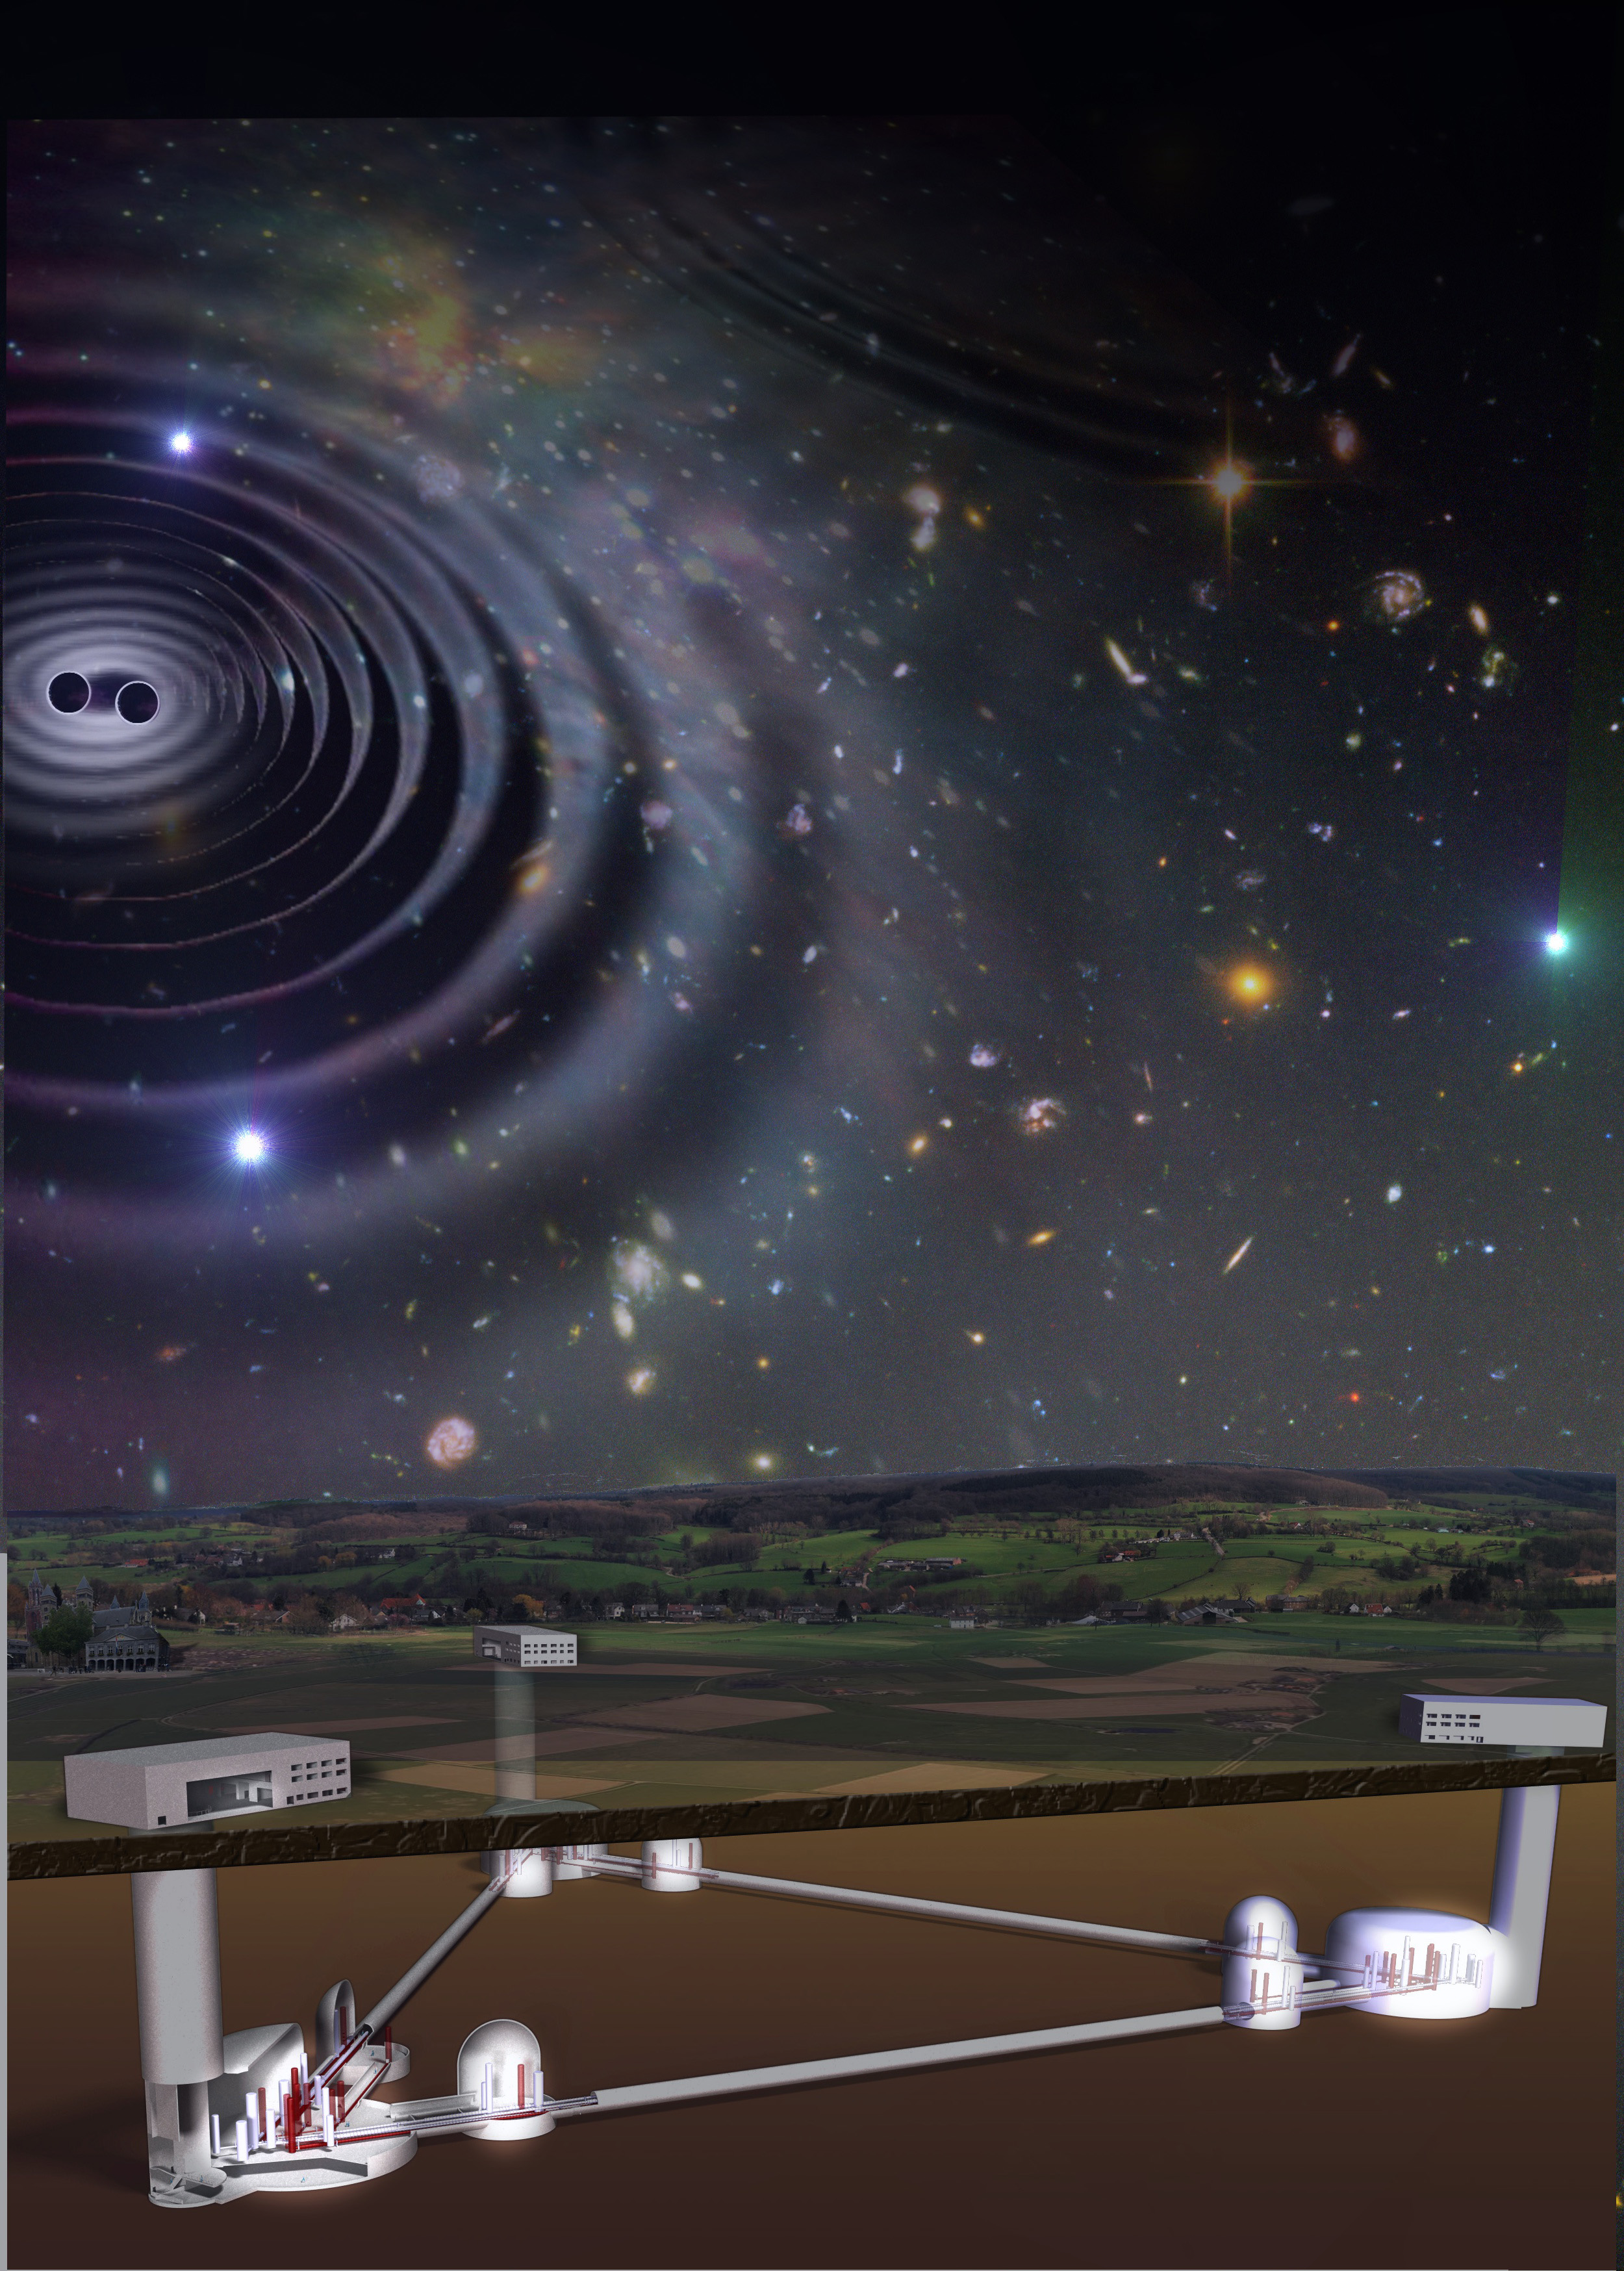
\includegraphics[width=0.7\textwidth]{Ca_Foscari Beamer/ETatNight2.jpg}
    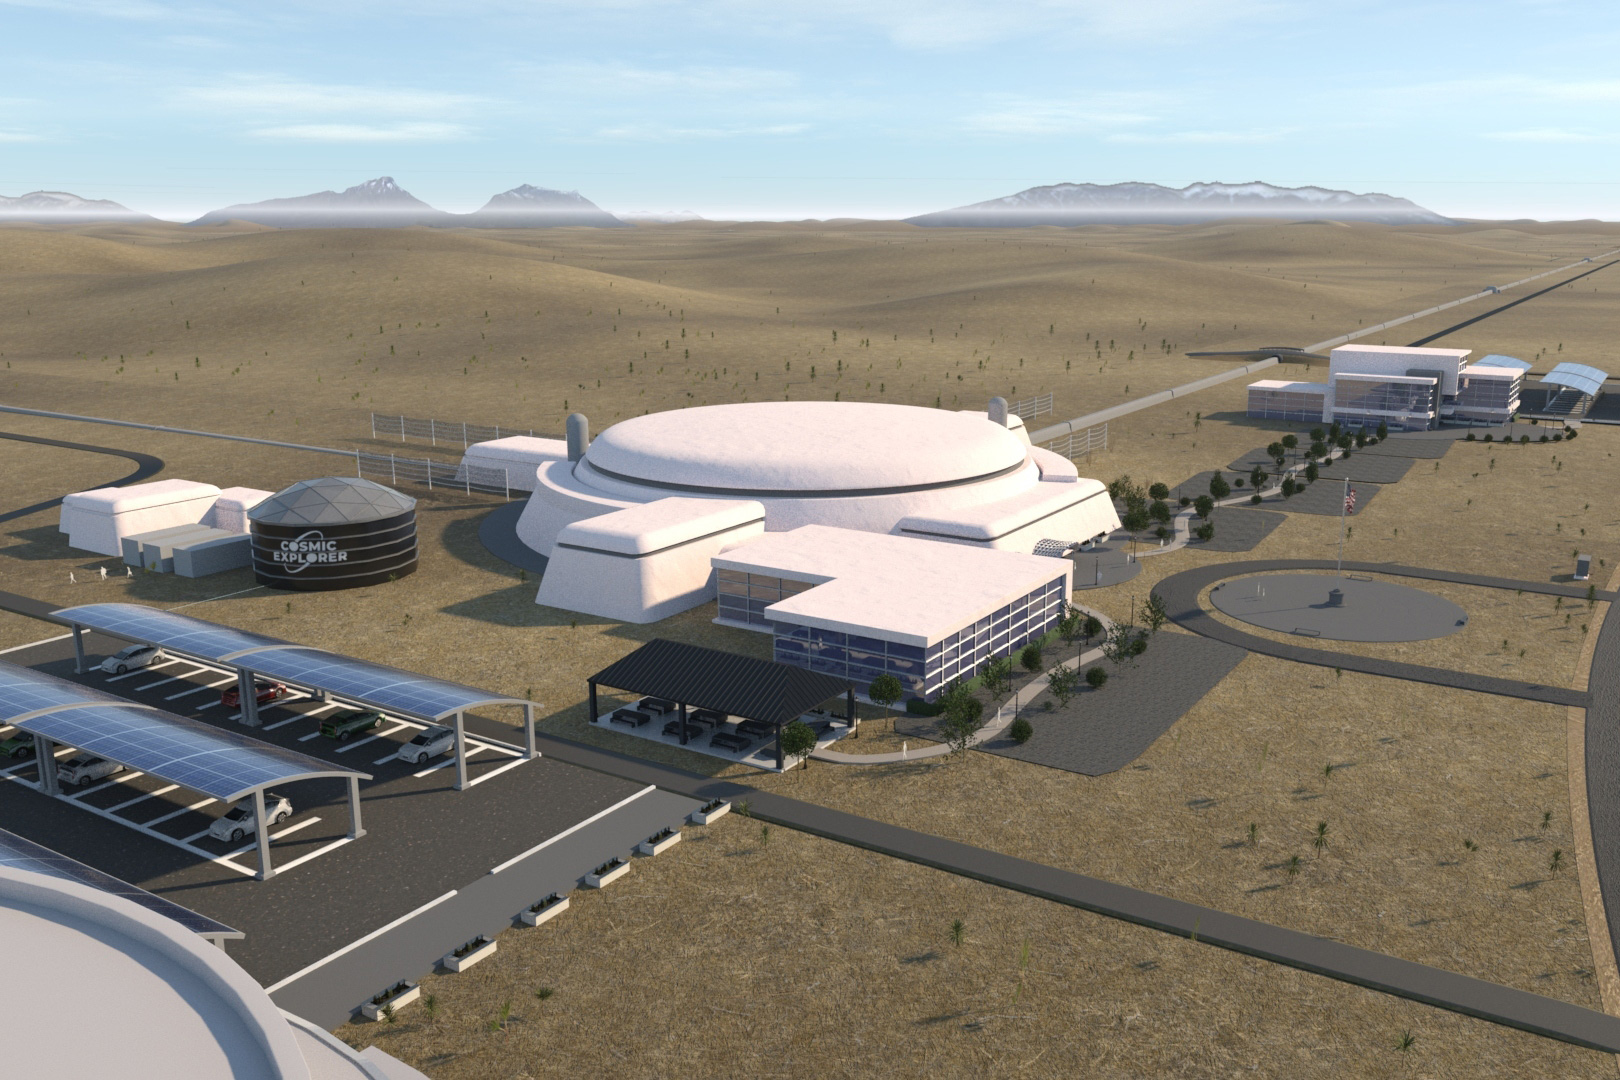
\includegraphics[width=0.7\textwidth]{Ca_Foscari Beamer/cosmicexplorer.jpg}
    
\end{columns}
\end{frame}

\begin{frame}{The data (space-based)}
    \begin{columns}
        \column{0.4\textwidth}
            \centering
            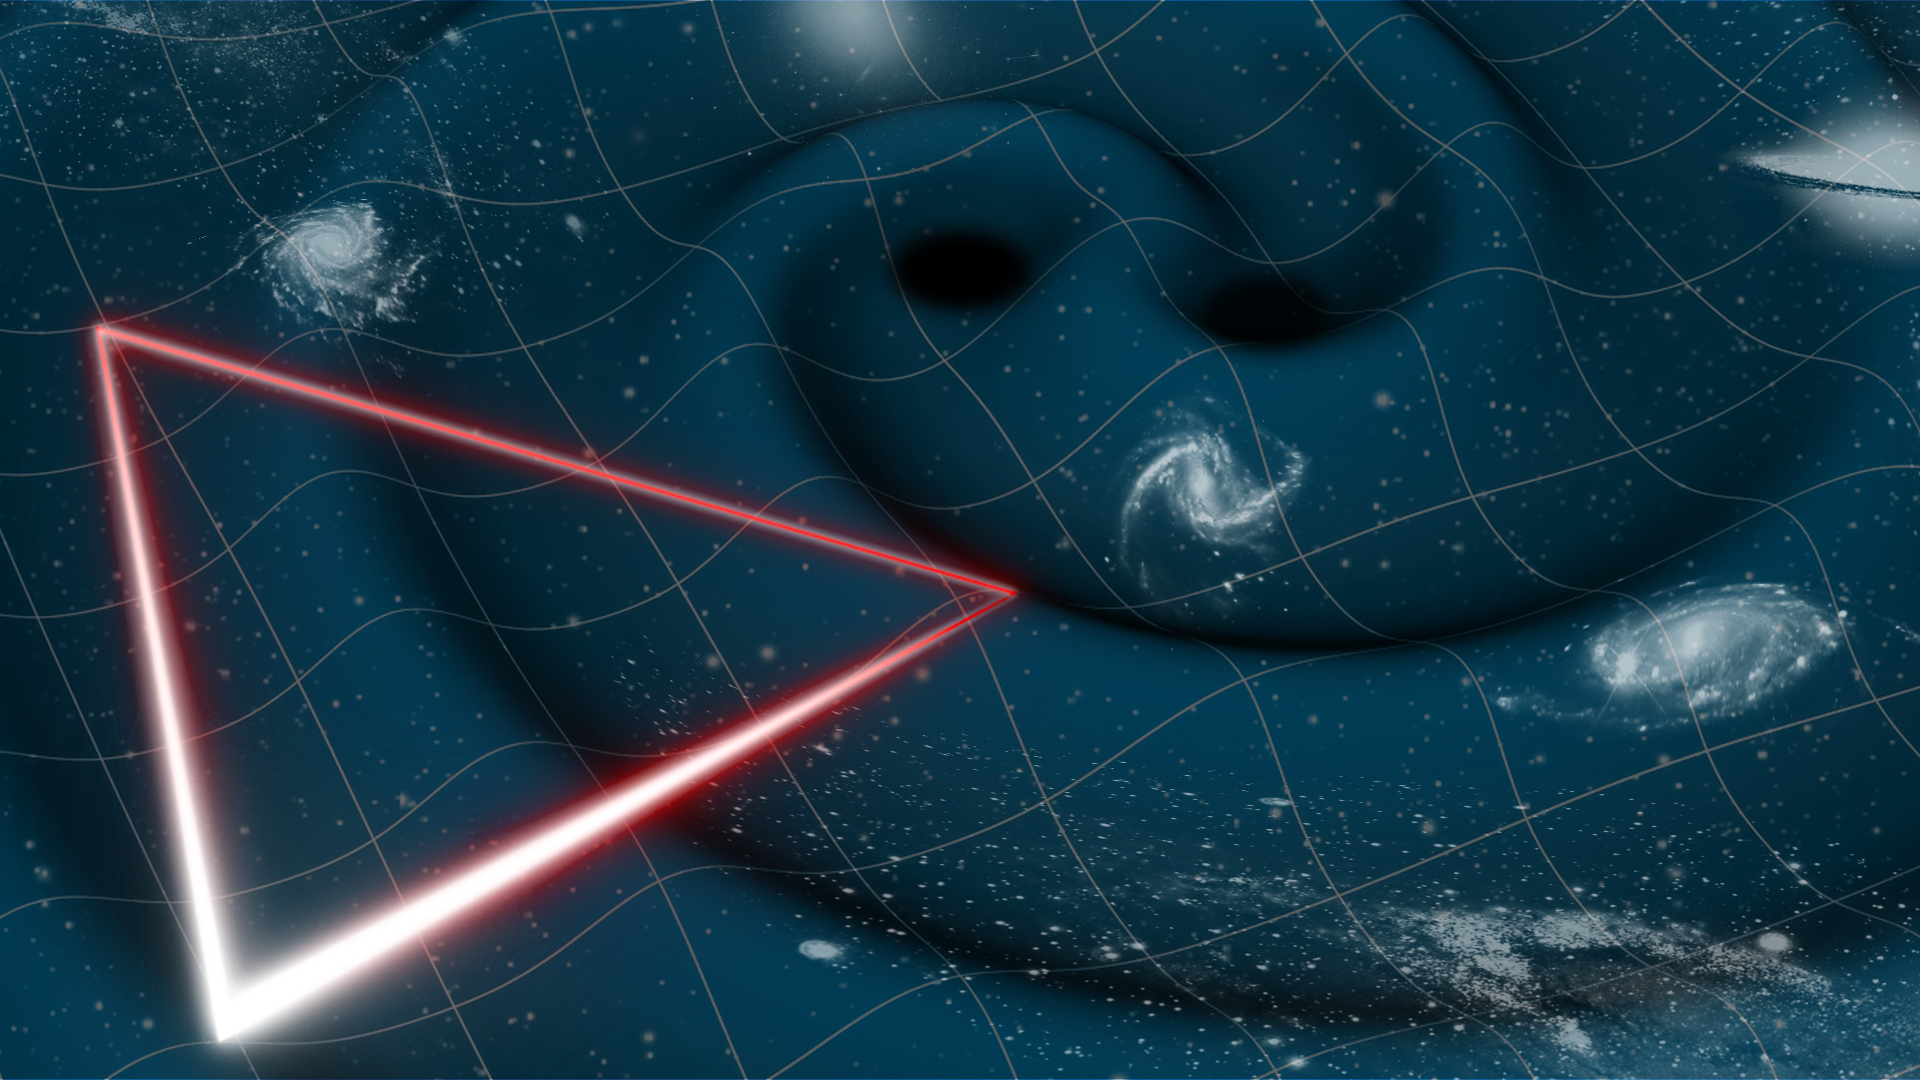
\includegraphics[width=\textwidth]{Ca_Foscari Beamer/LISA-inspired_artwork (1).png}
        \column{0.6\textwidth} \vspace{1cm}
        \bblock{\centering LISA}
            \begin{itemize}
                \item mHz frequency band
                \begin{itemize}
                    \item Galactic binaries, MBHBs, SOBHB, EMRIs %GBS most numerous, MHBHS strongest
                \end{itemize}
            \item Much higher SNRs
            \item Significantly longer signal durations %SMBHBs days to weeks, EMRIs for years
            \item Signal-dominated observatory
            \item Noise:
                \begin{itemize}
                    \item Non-stationary
                    \item Data gaps
                    \item Spacecraft motion
                \end{itemize}
            \end{itemize}
        \eblock
        
    \end{columns}
\end{frame}

\begin{frame}{Scaling of traditional methods}
Time of convergence of NS: {\tiny 2212.01760}
\vfill
    \begin{equation}
        T \propto \tikzmarknode{a1}{T_{\mathcal{L}}} \times \tikzmarknode{a2}{f_{\textrm{sampler}}} \times \tikzmarknode{a3}{D_{\textrm{KL}}} \times \tikzmarknode{a4}{n_{\textrm{live}}} 
    \end{equation}
    \begin{tikzpicture}[remember picture, overlay]
    \visible<2->{\draw[explain, <-, thick, firebrick](a4)--++(1.5,1)node[above]{resolution};}
    \visible<1->{\draw[explain, <-, thick, firebrick](a1)--++(-2,1)node[above]{likelihood evaluation time};}
    \visible<3->{\draw[explain, <-, thick, firebrick](a2)--++(-2.8,-1.7)node[below]{drawing new live point};}

    \onslide<3->{\node[anchor=south, inner sep=12pt] at (current page.south west) {\hspace{8em}
            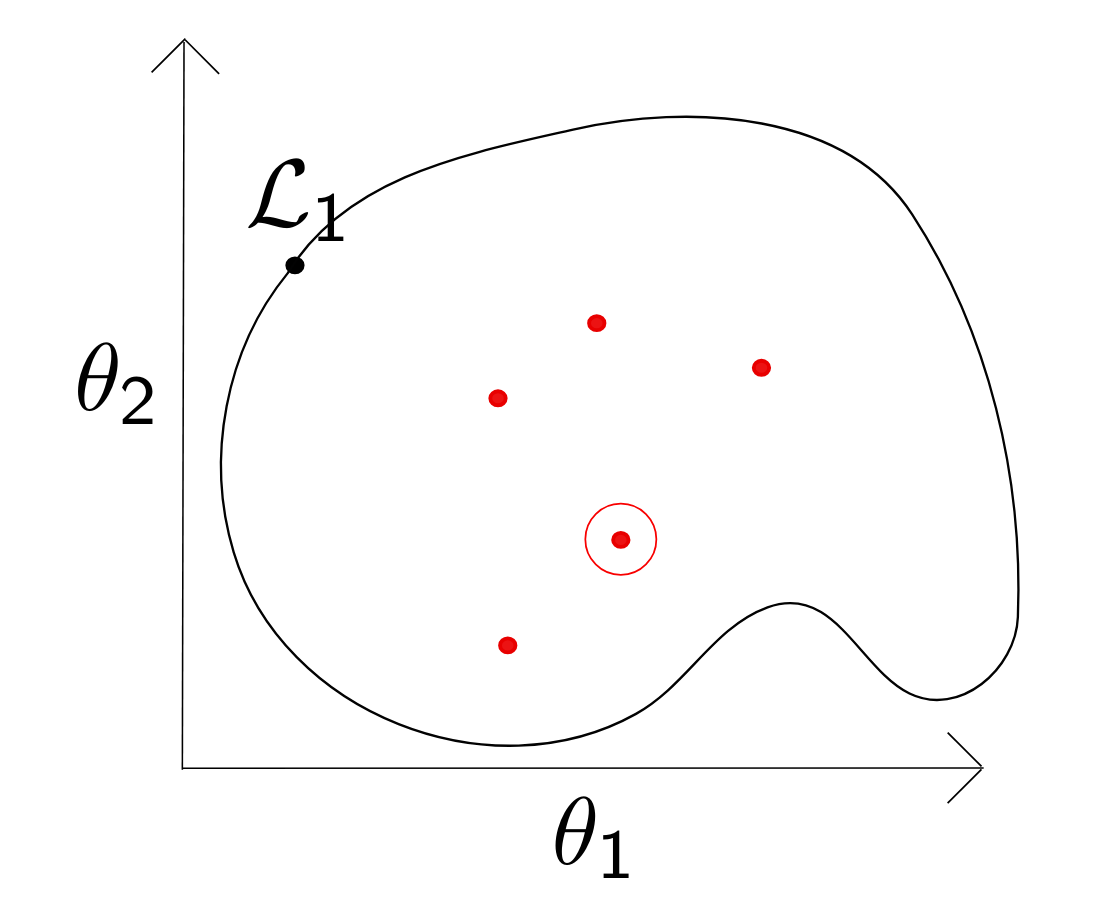
\includegraphics[width=0.2\textwidth]{Ca_Foscari Beamer/Screenshot from 2024-11-22 10-06-12.png}
        };}

    \onslide<4->{\node[anchor=south, inner sep=15pt] at (current page.south east) {\hspace{-8em}
        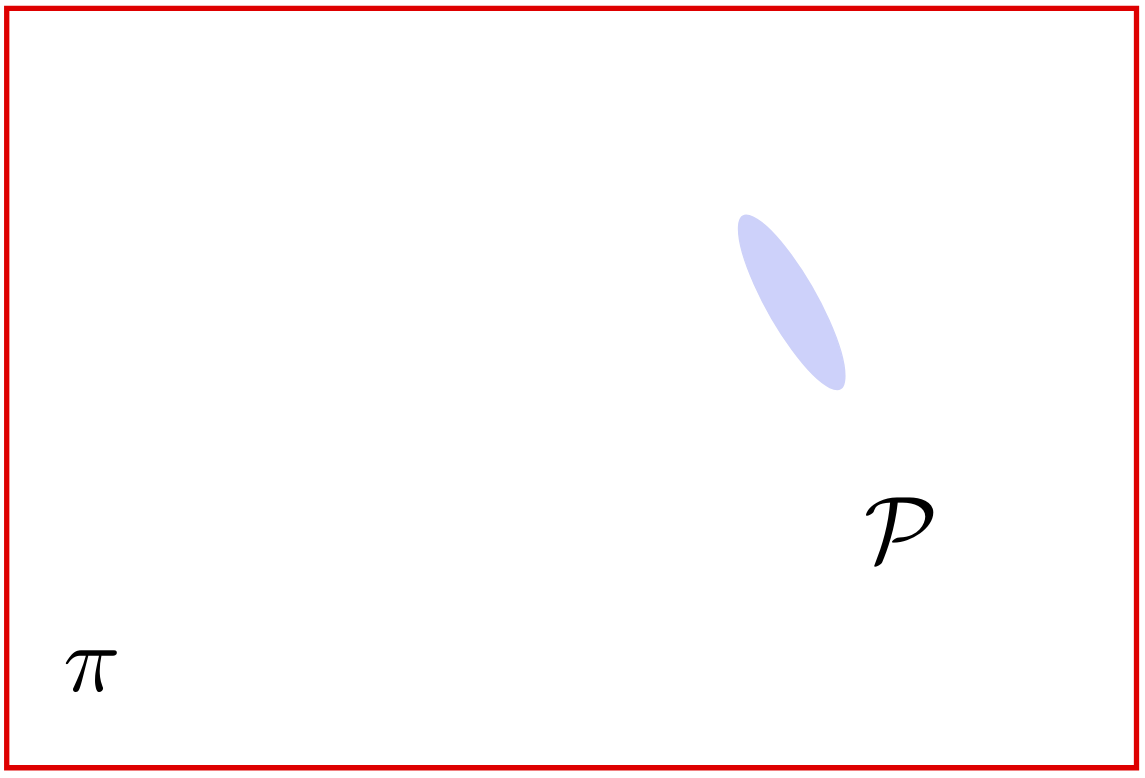
\includegraphics[width=0.17\textwidth]{Ca_Foscari Beamer/kl_div_screenshot.png}
    };}
        
    \visible<4->{\draw[explain, <-, thick, firebrick](a3)--++(1.2,-0.6)node[below]{compression from \textcolor{BurntOrange}{prior} to \textcolor{RoyalBlue}{posterior} ($\approx \mathrm{ln}\frac{V_\pi}{V_\mathcal{P}}$)};}
    \end{tikzpicture}
\end{frame}

% \begin{frame}{Scaling for model comparison}

% \begin{block}{Time of convergence of NS}
%     \begin{equation}
%         T \propto T_{\mathcal{L}} \times f_{\textrm{sampler}} \times D_{\textrm{KL}} \times n_{\textrm{live}} 
%     \end{equation}
% \end{block}
% \begin{block}{Uncertainty in log$\textcolor{red}{\mathcal{Z}}$}
%     \begin{equation}
%         \sigma \propto \sqrt{D_{\textrm{KL}} / n_{\textrm{live}}}
%     \end{equation}
% \end{block}

% \alert{Precision-normalized} runtime has quadratic dependence on KL divergence. \textcolor{cfgrey}{2212.01760}
% \end{frame}

\begin{frame}{Challenges with future data}
    \begin{equation}
        T_{\textrm{total}} \propto \tikzmarknode{N}{N_{\textrm{signals}}} \times \tikzmarknode{Tl}{T_{\mathcal{L}}} \times \tikzmarknode{a2}{f_{\textrm{sampler}}} \times  \tikzmarknode{DKL}{D_{\textrm{KL}}} \times \tikzmarknode{a4}{n_{\textrm{live}}} 
    \end{equation}

\begin{tikzpicture}[remember picture, overlay]
\visible<1->{\draw[explain, <-, thick, firebrick] (N)--++(-1,-1) 
    node[below]{higher sensitivity};}
    
\visible<2->{\draw[explain, <-, thick, firebrick] (DKL)--++(0.9,-0.7) 
    node[below]{higher SNR + longer signal $\Rightarrow$ narrower posterior};}

    \visible<3->{\draw[explain, <-, thick, firebrick] (Tl)--++(-2,1) 
    node[above]{longer signal duration $\Rightarrow$ slower waveform generation};}

    \visible<4->{\node (text) at (10.05, -0.8) {\textcolor{firebrick}{overlapping signals $\Rightarrow$ joint PE}};}


    \visible<5->{\node (L) at (3.75, 2.6) {\textcolor{firebrick}{overlapping signals $\Rightarrow$ joint likelihood}};}

    \visible<6->{\node (text2) at (10.55, -1.4) {\textcolor{firebrick}{duration $\gtrsim 10 \textrm{mins} \Rightarrow$ extra modeling}};} %earth's rotation, varying PSD

    \visible<7->{\node (text4) at (10.5, -2) {\textcolor{firebrick}{non-stationary noise}};}
    \visible<7->{\node (L) at (3.75, 3.1) {\textcolor{firebrick}{non-stationary noise}};}
    \visible<8->{\node (text3) at (7, -3) {\textbf{Billions to quadrillions of CPU core hours for 1 month of ET data...} \tiny 2412.02651};} %cite John Veitch

    
\end{tikzpicture}
\end{frame}

\begin{frame}{Established acceleration attempts}
\vfill
    \visible<1->{\begin{block}{Heterodyning}
        Exploits the smooth changes in GW waveforms near the maximum likelihood point. Assigns fiducial source parameter close to the true value and uses coarser frequency resolution. 
    \end{block}
    \begin{block}{Reduced Order Quadrature}
        Approximates the waveform model as a linear combination of a small number of pre-trained bases evaluated at representative frequencies. 
    \end{block}
    \begin{block}{Multibanding}
        Adjusts data resolution for gravitational wave signals across frequency bands, particularly during low-frequency early inspiral stage of CBCs. 
    \end{block}} \vfill
    \centering
    \visible<2->{\textbf{Even with these, millions of CPU core hours for 1 month of ET data.} \tiny 2412.02651}
\end{frame}

\section{Future of GW inference}

\begin{frame}{ML for traditional methods}
        \begin{equation}
        T \propto \tikzmarknode{a1}{T_{\mathcal{L}}} \times \tikzmarknode{a2}{f_{\textrm{sampler}}} \times \tikzmarknode{a3}{D_{\textrm{KL}}} \times \tikzmarknode{a4}{n_{\textrm{live}}} 
    \end{equation}
    \begin{tikzpicture}[remember picture, overlay]
    % \visible<2->{\draw[explain, <-, thick, firebrick](a4)--++(1.5,1)node[above]{resolution};}
    \visible<1->{\draw[explain, <-, thick, firebrick](a1)--++(-2,1)node[above]{ROM, surrogates};} % artificial neural networks to map gravitational-wave source parameters into basis coefficients
    \visible<2->{\draw[explain, <-, thick, firebrick](a2)--++(-2.8,-1.7)node[below]{\textsc{nessai}};}

    \onslide<2->{\node[anchor=south, inner sep=12pt] at (current page.south west) {\hspace{8em}
            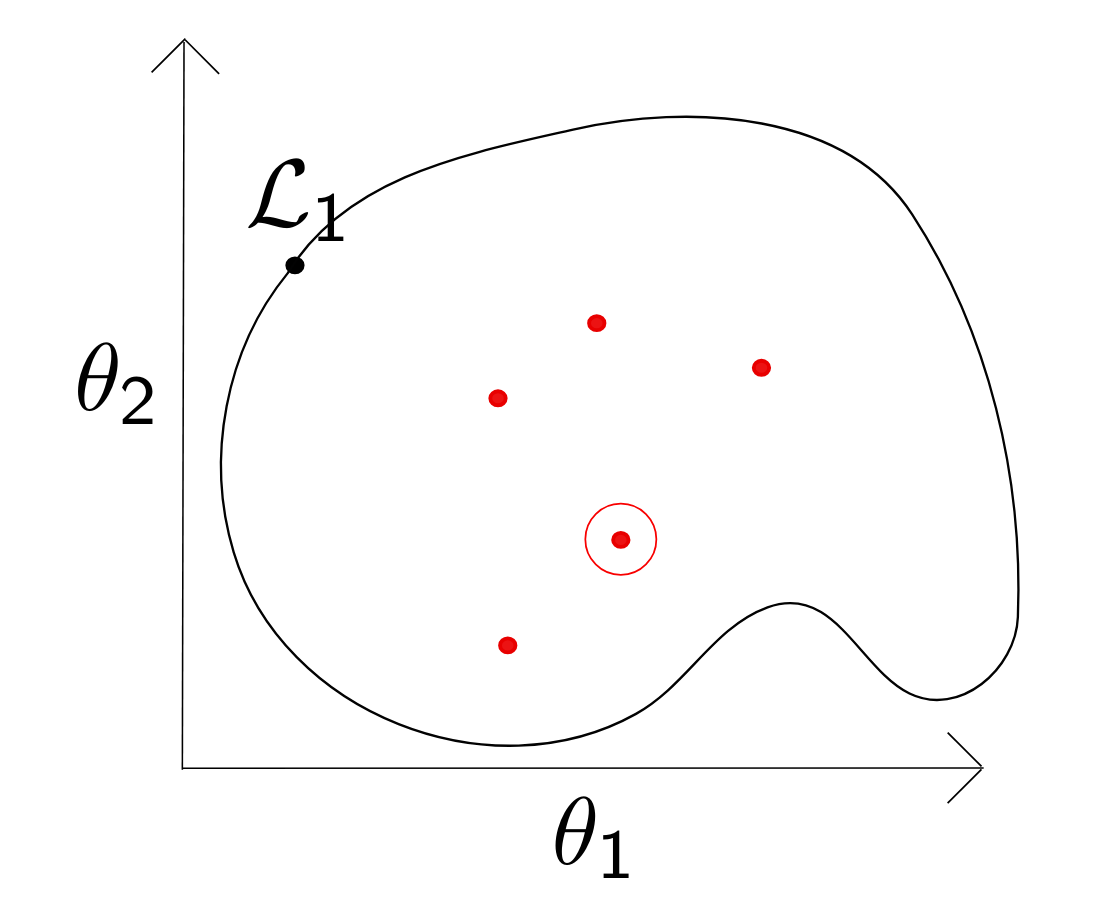
\includegraphics[width=0.2\textwidth]{Ca_Foscari Beamer/Screenshot from 2024-11-22 10-06-12.png}
        };}

    \onslide<3->{\node[anchor=south, inner sep=15pt] at (current page.south east) {\hspace{-8em}
        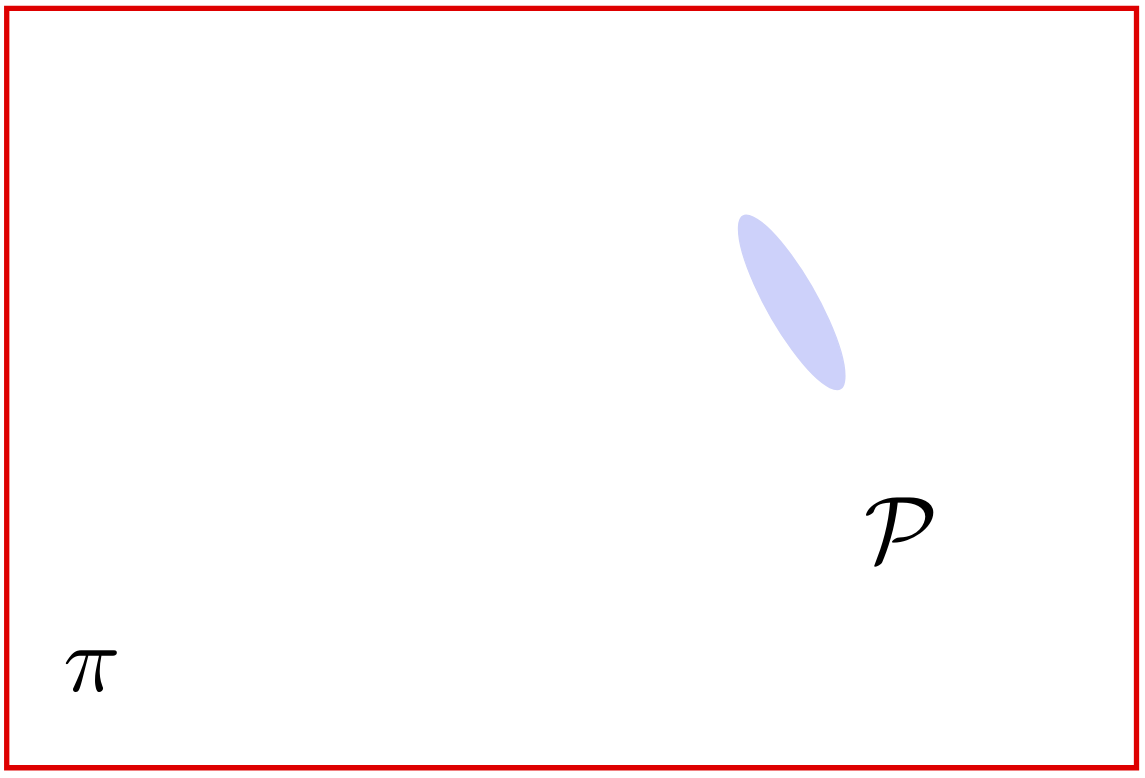
\includegraphics[width=0.17\textwidth]{Ca_Foscari Beamer/kl_div_screenshot.png}
    };}
    \visible<3>{\draw[explain, <-, thick, firebrick](a3)--++(1.2,-0.6)node[below]{not as baked-in as you might think!};}
    \visible<4->{\draw[explain, <-, thick, firebrick](a3)--++(1.2,-0.6)node[below]{posterior repartitioning with $\beta$-flows};}
    \end{tikzpicture}
    % Have only just begun to set benchmarks for acceleration methods for 3G era - lots more to be done here to study the speedups we can expect.
\end{frame}

\begin{frame}{SBI}
    \begin{columns}
        \column{0.6\textwidth}
        \vspace{0.5cm}
        \visible<1->{\bblock{Simulation Based Inference}
            \begin{itemize}
                \item Generate `simulations' (forward model) to do inference %draw theta, simulate D
                \begin{itemize}
                    \item Draw $\theta$ from prior, simulate $D$
                    \item Use NPE, NLE, NRE to evaluate $p(\theta|D_0)$
                \end{itemize}
                \item No explicit likelihood
                \item Potentially amortizable
                \item Examples for GWs: 
                \begin{itemize}
                    \item \textsc{DINGO} (NPE, amortized)
                    \item \textsc{PEREGRINE} (TMNRE, sequential)
                \end{itemize}
                \item Doesn't require ML (see e.g. \textsc{LSBI}), but ML has driven significant advances.
            \end{itemize}
        \eblock}

        \column{0.4\textwidth}
        \vspace{0.3cm}
        \visible<2->{\begin{block}{Advantages for 3G + LISA era}
            \begin{itemize}
                \item Overlapping signals, non-stationary noise, stochastic backgrounds complicate likelihood
                \item Almost real-time inference if amortized $\Rightarrow$ EM follow-up
                \item More simulation-efficient $\Rightarrow$ higher fidelity waveform models
                \item Well-suited for catalog-level tasks
            \end{itemize}
        \end{block}}
        
    \end{columns}
\end{frame}

\begin{frame}{GPUs}
    \begin{itemize}
        \item Parallel processing power of GPUs can speed up Bayesian inference by factor of thousands
        \item \textsc{ripple}: \textsc{jax} implementation of models for GPU-accelerated waveform calls
        \item \textsc{jim} uses \textsc{ripple} + \textsc{flowMC}
    \end{itemize}
    \vspace{1cm}
    \visible<2->{
    \bblock{\centering \textsc{blackjax NS}}
        \begin{itemize}
            \item Nested sampling implementation in \textsc{blackjax}
            \item 11 parameter nested sampling run on GW150914 in minutes
        \end{itemize}
    \eblock
    }
\end{frame}

\begin{frame}{Conclusions}
    % Frontiers of GW PE are machine learning, SBI, GPUs. All of these are being developed in some form by the Cambridge community, meaning lots of exciting research and avenues for collaboration!
    \begin{itemize}
        \item 3G + LISA era presents significant challenges for data analysis
        \item Current standard inference methods will not scale well
        \item ML-accelerated sampling, SBI and GPU-accelerated pipelines will work towards addressing these challenges
    \end{itemize}
\end{frame}


%---------------------------------------------------------


\end{document}
